\documentclass{article}
\usepackage[utf8]{inputenc}
\usepackage[english]{babel}
\usepackage{url,graphicx,tabularx,array,geometry}
\usepackage{tabularx}
\usepackage{pgfplots}
\usepackage{amsmath}
\usepackage{amsfonts}
\usepackage{amssymb}

\title{Intelligent Patient Record}

\author{ITU \\
\vspace{5mm}
Mathias Schmidt, Thomas Snaidero \\
Supervisors: \\
Steven Houben, Mads Frost}

\date{21 May 2014}

\begin{document}

\maketitle
\pagebreak
\tableofcontents
\pagebreak


\section{Introduction}


We have had the task of build a new revision, of Steven Houben Hyper Record.

One of the big reasons is it was to unwieldy and heavy for the medical staff.


\section{Design requirements}

Houben et al.'s proposed device shown on figure \ref{fig:old-hypr} was taken as a reference, with regards to weight, thickness and size. Although the new design retains the same purpose, the feature of having a dock for a tablet was removed, to further reduce the size. The hybrid patient record was then re-imagined to be just a thin support for a folder, with electronics on the back. \\

Working from Houben et al.'s proposed device, a new set of requirements have been established, in order to improve on the design. The following is a list of requirements pertaining to the new device:

\begin{itemize} \itemsep0em
	\item Weight: less than 500g
	\item Thickness: less than 20mm
	\item Size: Approximately same dimensions as A4 paper
	\item Maintainability: easy access to the microcontroller's programming interface
	\item Maintainability: easily change components without changing physical design
\end{itemize}

A set of requirements pertaining to the electronic part of the device has also been decided:

\begin{itemize} \itemsep0em
	\item Rechargeable battery via standard USB cable
	\item Battery status LEDs
	\item Autonomy of at least 8 hours on battery, with normal use
	\item LEDs showing colour combinations should be easily seen and understood from 10m 
	\item Hear the audio signal in a room, when device is under bed sheets
\end{itemize}

\begin{figure}[h]
\begin{center}
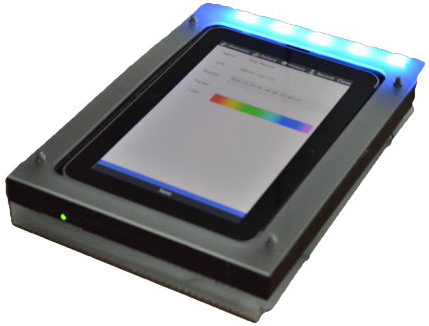
\includegraphics[scale=.5]{figures/old-hypr.jpg}
\caption{\small {\it {This is a description}}} \label{fig:old-hypr}
\end{center}
\end{figure}
% Numbered list of product requirements with most important first, least important last.

\section{Use case scenarios}
% Detailed description of 3 use case scenarios which illustrate:
% - The user experience
% - Insight about a specific product feature, or user requirement

\section{Design analysis and concept diagrams}
Description of issues related to the design of the product:
- Description of concepts, requirements and features of the product
- Review of motivations for making the design decisions
- Indicate the primary features of the design that are the most creative and original

\subsection{Materials}
We got a bunch of different plast materials from RIAS, in order to find some material that might be cheaper, and better that acrylic, since acrylic have tendency to be brittle, this becomes worse when it has been laser cut. 
PEHD
RIALEN PP
PETG
PP-H
ACRYL
POM-C

PEEK
PPSU

\subsection{Iterations}
we have used prototyping in order to get a viable device, through the different designs we have been able to see different problems, which have ment that we had to iterate to a new version, we have been limited by time, so we have had to make some compromises

\subsubsection{fisrt}
The first iteration that we build did have some problems.
The first is that it is expensive to build, since we are using a lot of acrylic, the secound point is that it still is heavy, and unwieldy.
But i did give some ideas for the next iteration.

\subsubsection{secound}


\subsubsection{thried}


\subsubsection{fourth}


\subsubsection{fith}

\subsubsection{sixth}


% Description of issues related to the design of the product:
% - Description of concepts, requirements and features of the product
% - Review of motivations for making the design decisions
% - Indicate the primary features of the design that are the most creative and original

\section{Prototyping analysis}

Discussion of experience in building prototypes during the design process:
- Illustration of all the prototyping activities
- Discussion of specific areas where the experience of building prototypes affected the design requirements and specifications
% Discussion of experience in building prototypes during the design process:
% - Illustration of all the prototyping activities
% - Discussion of specific areas where the experience of building prototypes affected the design requirements and specifications



% Explanations of how to build the product, including information such as:
% - System architecture
% - Drawings and sketches
% - Parts and supply ordering information

% Design specifications marked for:
% - Quality
% - Accuracy
% - Originality

\section{TESTING - ignore}

\begin{figure}[h]
\begin{center}
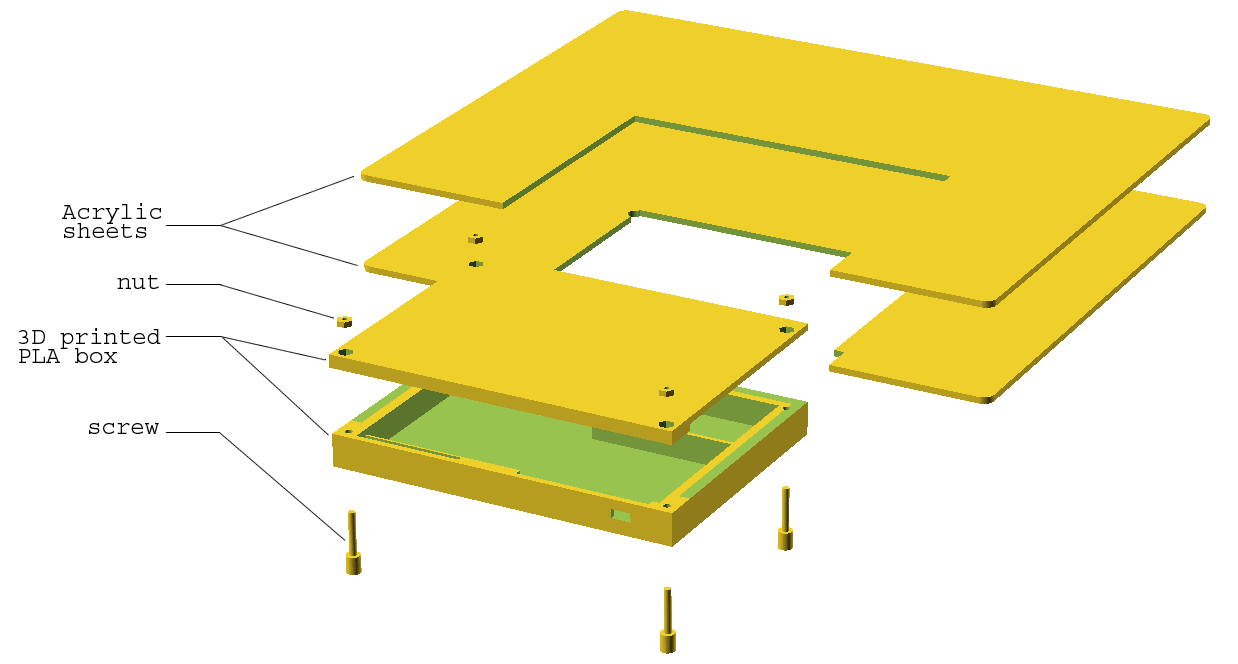
\includegraphics[scale=0.5]{figures/explode.png}
\caption{\small {\it {This is a description}}} \label{fig:explode}
\end{center}
\end{figure}


\begin{figure}[h]
\begin{minipage}[b]{7.5cm}
\centering
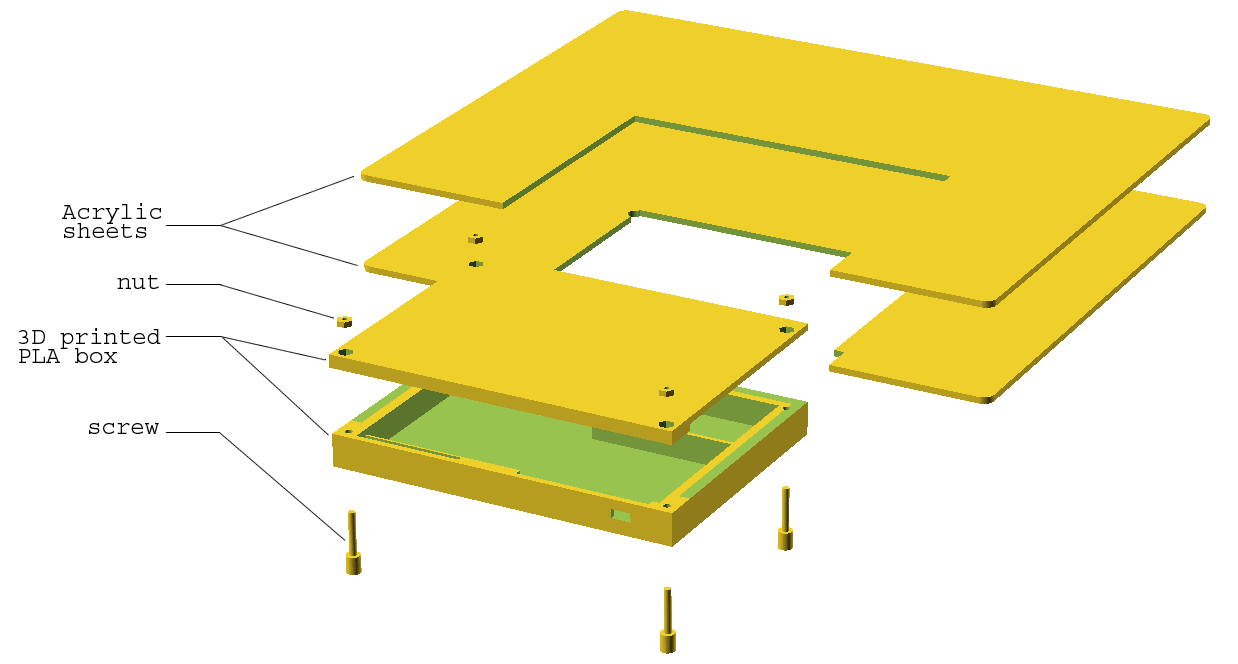
\includegraphics[scale=0.20]{figures/explode.png}
\caption{\small {\it {This is a description}}} \label{fig:testfig1}
\end{minipage}
\hspace{0.5cm}
\begin{minipage}[b]{7.5cm}
\centering
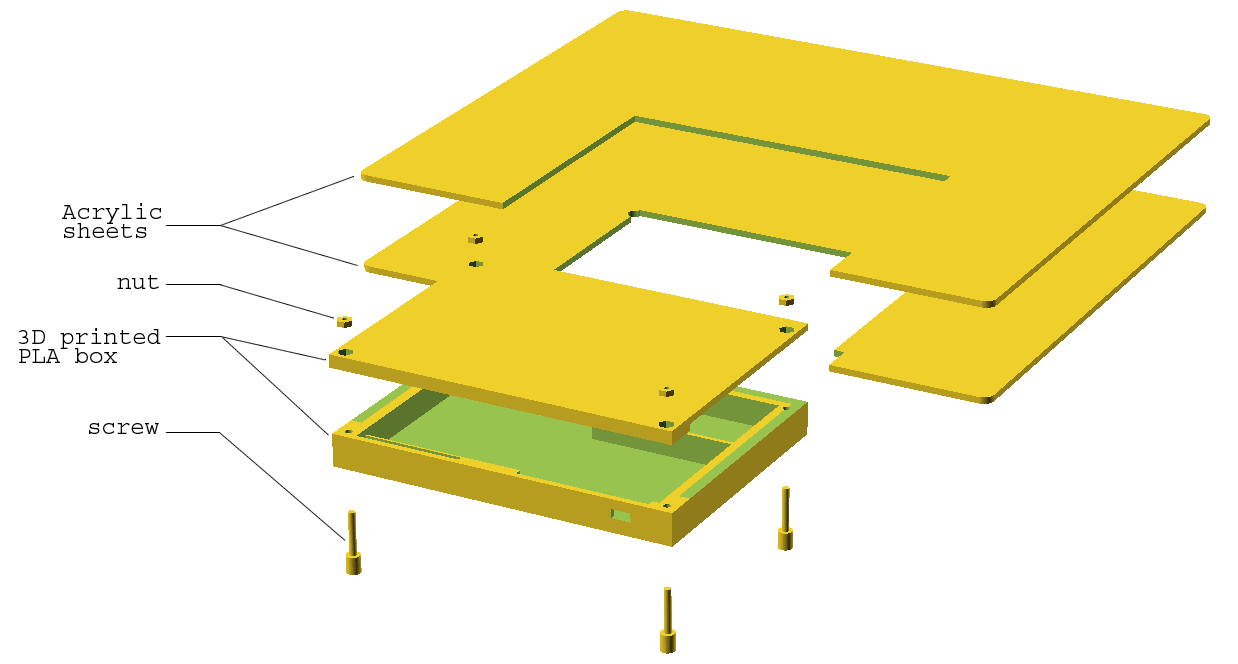
\includegraphics[scale=0.20]{figures/explode.png}
\caption{\small {\it {This is a description}}} \label{fig:testfig2}
\end{minipage}
\end{figure}


\begin{itemize} \itemsep0em
  \item The individual entries are indicated with a black dot, a so-called bullet \cite{chua2010}.
  \item The text in the entries may be of any length.
\end{itemize}


\section{Conclusions}



% \section{Electronic}

\title{Electronic}



% \section{Design}
\subsection{Materials}
We got a bunch of different plast materials from RIAS, in order to find some material that might be cheaper, and better that acrylic, since acrylic have tendency to be brittle, and this becomes worse when it has been laser cut. 

\subsection{Iterations}
we have used prototyping in order to get a viable device, through the different designs we have been able to see different problems, which have ment that we had to iterate to a new version, we have been limited by time, so we have had to make some compromises

\subsubsection{fisrt}
The first iteration that we build did have some problems.
The first is that it is expensive to build, since we are using a lot of acrylic, the secound point is that it still is heavy, and unwieldy.
But i did give some ideas for the next iteration.

\subsubsection{secound}


\subsubsection{thried}


\subsubsection{fourth}


\subsubsection{fith}



% \section{Problems}









\end{document}


%-----------------------------------------------
% Resources

http://www.me.umn.edu/education/undergraduate/writing/How-to-write-a-Design-Report.pdf

http://pastebin.com/raw.php?i=xudGnU7U

http://ocw.mit.edu/courses/sloan-school-of-management/15-783j-product-design-and-development-spring-2006/index.htm

